\subsection{Introduction}
\textbf{Spike Sorting} can be defined as the grouping of spikes into clusters according
to the similarity of their shapes.\\
It is useful only if the following assumption is made: each neuron tends to fire spikes
with a peculiar (distinguishable) extracellular shape.
As a consequence, it is possible to determine the activity of each one of these neurons
according to the measured spikes associated with it through Spike Sorting.\\
There are 3 main reasons for which Spike Sorting useful:
\begin{itemize}
    \item \textbf{Increase the scale}: as modern devices (MEAs) record from large
          populations of neurons at the same time, it is desirable to derive the individual
          activity of as many neurons as possible.
    \item \textbf{Carry out new types of analysis}: it might be interesting to study
          connectivity patterns of close-by neurons or perform analysis at single-neuron
          level.
    \item \textbf{Have access to sparsely firing neurons}: it is desirable to understand
          the typical patterns of a specific kind of neuron, allowing to study its specific
          function.
\end{itemize}
Despite everything, Spike Sorting still presents a number of major problems:
\begin{itemize}
    \item Dealing with background noise.
    \item Neurons in the same area might produce spikes with a similar shape (there is
          no way to perfectly know which neuron fired apart from imaging techniques).
    \item Neurons in the same area might emit spikes with a smaller amplitude.
    \item Background activity of distant neurons pollutes the recorded signal.
    \item Waveform misalignment.
    \item Variation of the spike shape as a function of recent firing history
          (not time-invariant shape).
\end{itemize}
\begin{figure}[H]
    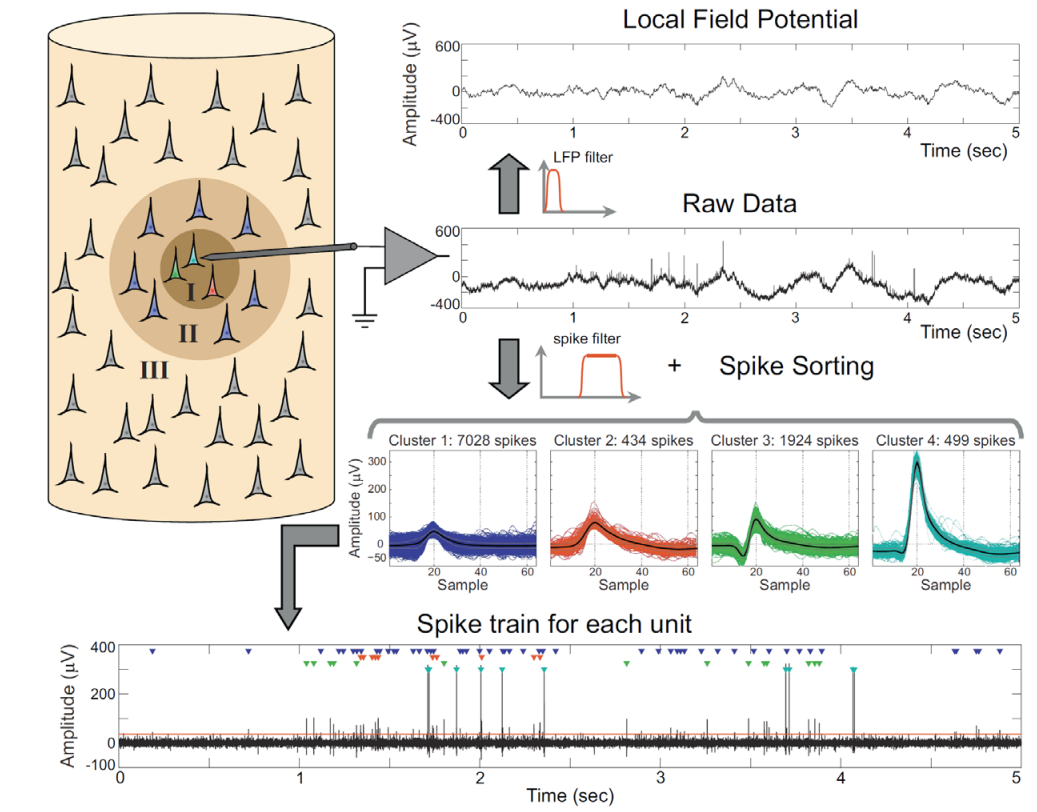
\includegraphics[scale=0.35]{3_1}
    \centering
\end{figure}

\subsection{Spike Sorting methods}
When it comes to Spike Sorting, there are three main approaches:
\begin{itemize}
    \item \textbf{Amplitude discriminator}: separate spikes according to their amplitude.
          This method does not take into account the shape of a spike, only its amplitude.\\
          \textit{Main problem:} spikes from different neurons may have the same peak
          amplitude but different shapes.
    \item \textbf{Template matching}: select a characteristic spike shape for each
          cluster and divide the spikes among the clusters via matching with the templates,
          according to an appropriate distance measure.\\
          \textit{Main problems:} the templates might need to be adjusted during the
          experiment and it is necessary a good way to select them in the first place.
    \item \textbf{Window discriminator}: assign spikes crossing one or more windows to
          the same neurons.\\
          \textit{Main problem:} it requires manual setting by the user and it is not
          suitable for many channels and subjectivity. Moreover, spikes may overlap: it may
          be difficult to set windows for discrimination and sparsely firing neurons may be
          missed.
\end{itemize}
Please note that these algorithms perform Spike Detection and Spike Sorting at the same
time.\\

\subsection{Spike Sorting steps}
In general, Spike Sorting is carried out by following the steps shown below:
\begin{figure}[H]
    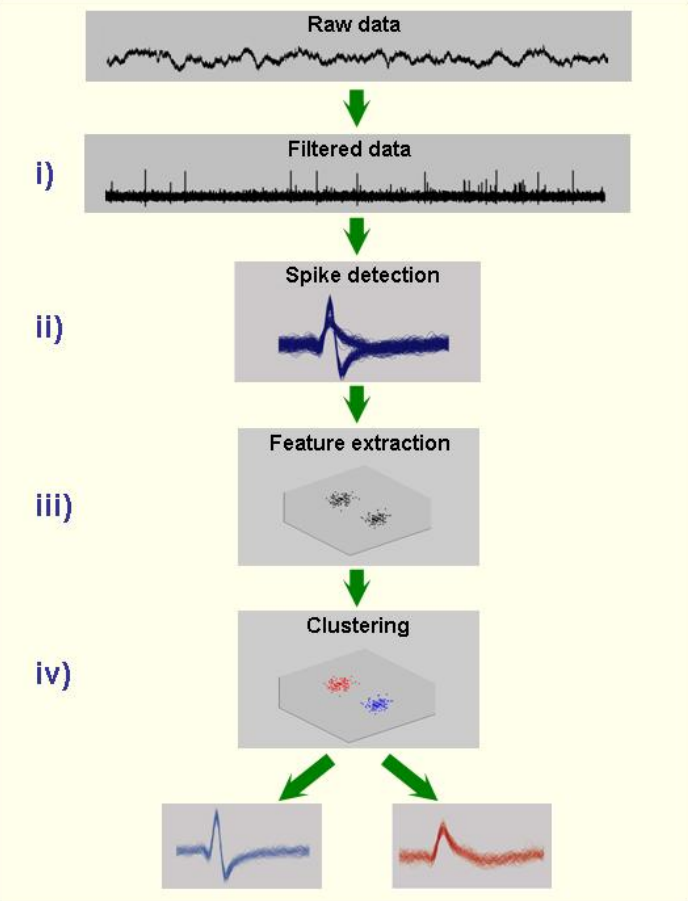
\includegraphics[scale=0.4]{3_2}
    \centering
\end{figure}
\subsubsection{Filtering}
The first step consists in filtering out the low frequency components (\(< 300 \,Hz\)),
in particular the local field potentials, in order to visualize spikes. To do so, a
\(300-3000 \,Hz\) band-pass filter is employed: all the frequencies outside the
specified range are rejected.
\begin{figure}[H]
    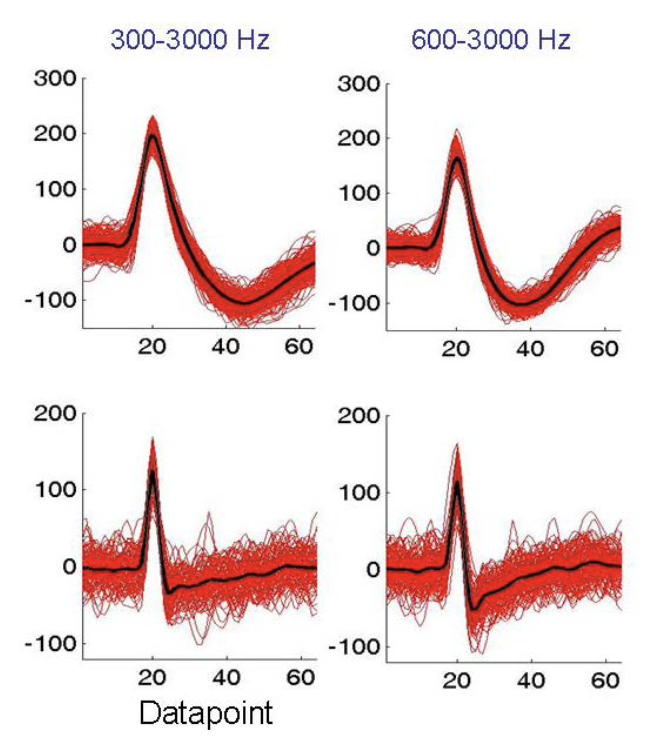
\includegraphics[scale=0.4]{3_3}
    \centering
\end{figure}
\subsubsection{Spike Detection}
Spikes are commonly detected by using an amplitude threshold, as seen in the previous
chapter. The optimal threshold can be set manually or automatically computed as a
multiple of the standard deviation \(\sigma\) of the signal:
\begin{equation*}
    \sigma=median\biggl(\frac{|x|}{0.6745}\biggr)
\end{equation*}
\subsubsection{Feature Extraction}
Let's set the number of observations - i.e. spikes - to \(n\) and the variables
(data points) to \(m\), thus a \(m\)-dimensional space is obtained. The idea is to
extract a number of features \(p\), such that \(p<m\). In this way the signal is
described with a decreased number of features with respect to the original ones.\\
The \(p\) features can be selected by:
\begin{itemize}
    \item Taking some basic properties of the spikes (amplitude, width, energy, ...),
          but they might not be optimal in differentiating spikes.
    \item Selecting a low number of components from a dimensionality reduction
          technique, such as \textbf{PCA}. Notice that these components represent the
          directions of maximum variance of the data, not necessarily the best separation.
    \item Using \textbf{wavelets}, obtaining a time-frequency decomposition of the
          signal with optimal resolution in both time and frequency domains.
\end{itemize}
\paragraph{Principal Component Analysis (PCA)}
It is an unsupervised dimensionality reduction technique, which can be used also for
feature extraction purposes. Data are rotated according to a new space having the
orthogonal axes in the directions of maximum variance, then the new obtained principal
components are ordered by their contribution to the overall variance, allowing to
select only a fraction of the total number of components, still approximating the
original data fairly well. Low variance is often interpreted as background noise.\\
The dimensionality of the data can therefore be reduced, without the loss of relevant
information, by extracting a lower dimensional space still ensuring a fairly high variance.
\begin{figure}[H]
    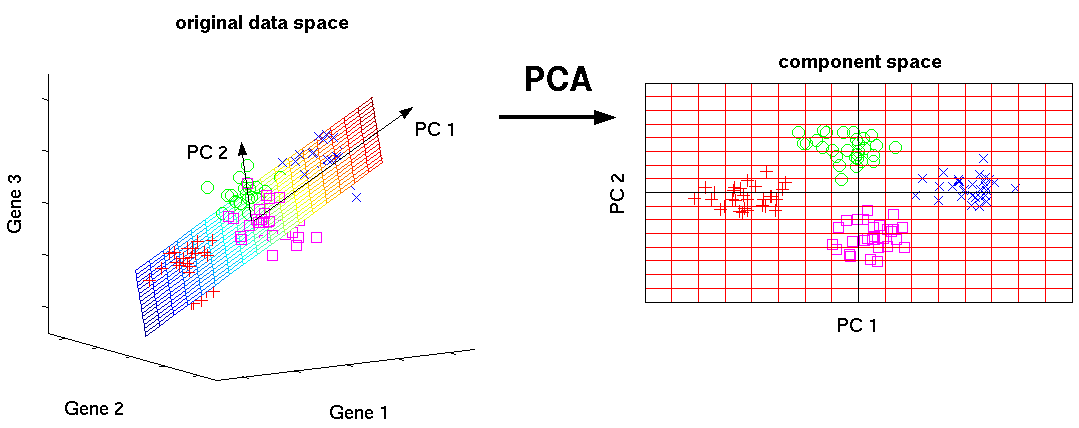
\includegraphics[scale=0.45]{3_4}
    \centering
\end{figure}
\paragraph{Wavelets}
The wavelet transformation (WT) is a joint time-frequency representation of the signal.
When compared to other more spread methods, it has the main advantage to provide an
optimal resolution in both the time and the frequency domains.\\
The wavelet analysis is similar to the windowed Fourier analysis in the sense that it breaks a
signal down into its constituent parts. However, whereas the Fourier transform breaks the
signal into a series of sine waves of different frequencies, the wavelet transform breaks
the signal into its wavelets, which are scaled and shifted versions of a parametric "mother"
wavelet. Notice that sines and cosines are infinite in time, while a wavelet must exhibit
a local support, indicating that it is finite in time.\\
The Wavelet transform may be defined as the convolution between the signal \(x(t)\) and the
wavelet function \(\psi_{a,b}(t)\):
\begin{align*}
    W_\psi X(a,b)=\left\langle x(t)|\psi_{a,b}(t) \right\rangle\hspace{0.5cm}\text{with}\hspace{0.5cm}\psi_{a,b}(t)=|a|^{-\frac{1}{2}}\psi\biggl(\frac{t-b}{a}\biggr)
\end{align*}
where \(a\) and \(b\) are scale and translation parameters.\\
A tight wavelet function will match the high-frequency components, while a dilated wavelet
will match the low-frequency ones, thus details of the signal at several scales are obtained.
\begin{figure}[H]
    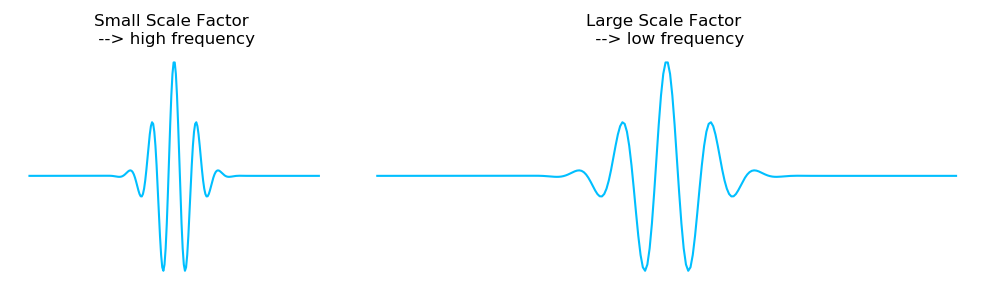
\includegraphics[scale=0.25]{3_5}
    \centering
\end{figure}
When employing wavelets, the information about the shape of the spikes is distributed
in several coefficients, not just in 2-3 PCs as it happens for PCA. A wavelet
coefficient (or any other feature) in order to be effective in distinguishing spike
shapes should have a multi-modal distribution, unless there is only one cluster.
\subsubsection{Clustering}
The final step of spike sorting consists in grouping together the spikes with similar
features into clusters, corresponding to different neurons. Different approaches are
available:
\begin{itemize}
    \item Manual clustering
    \item Bayesian classification
    \item Expectation-Maximization methods
    \item Hierarchical clustering
    \item K-Means
    \item Superparamagnetic clustering
\end{itemize}
\paragraph{K-means Clustering}
K-means clustering is a partitioning method that treats each observation in the data as
an object having a location in the space. It finds a partition in which objects within
each cluster are as close as possible, while object in different clusters should be as
far apart as possible.\\
Each cluster in the partition is defined by its members and by its centroid.
The centroid of each cluster is computed as the mean position of all the cluster members,
which are partitioned among the available clusters in order to minimize the sum of
the distances from the centroid itself.\\
It is quite important that the user sets the correct number of  desired clusters
(initial centroids can be specified as well).\\
Notice that this method works well with spherical and similarly scattered clusters.
\begin{figure}[H]
    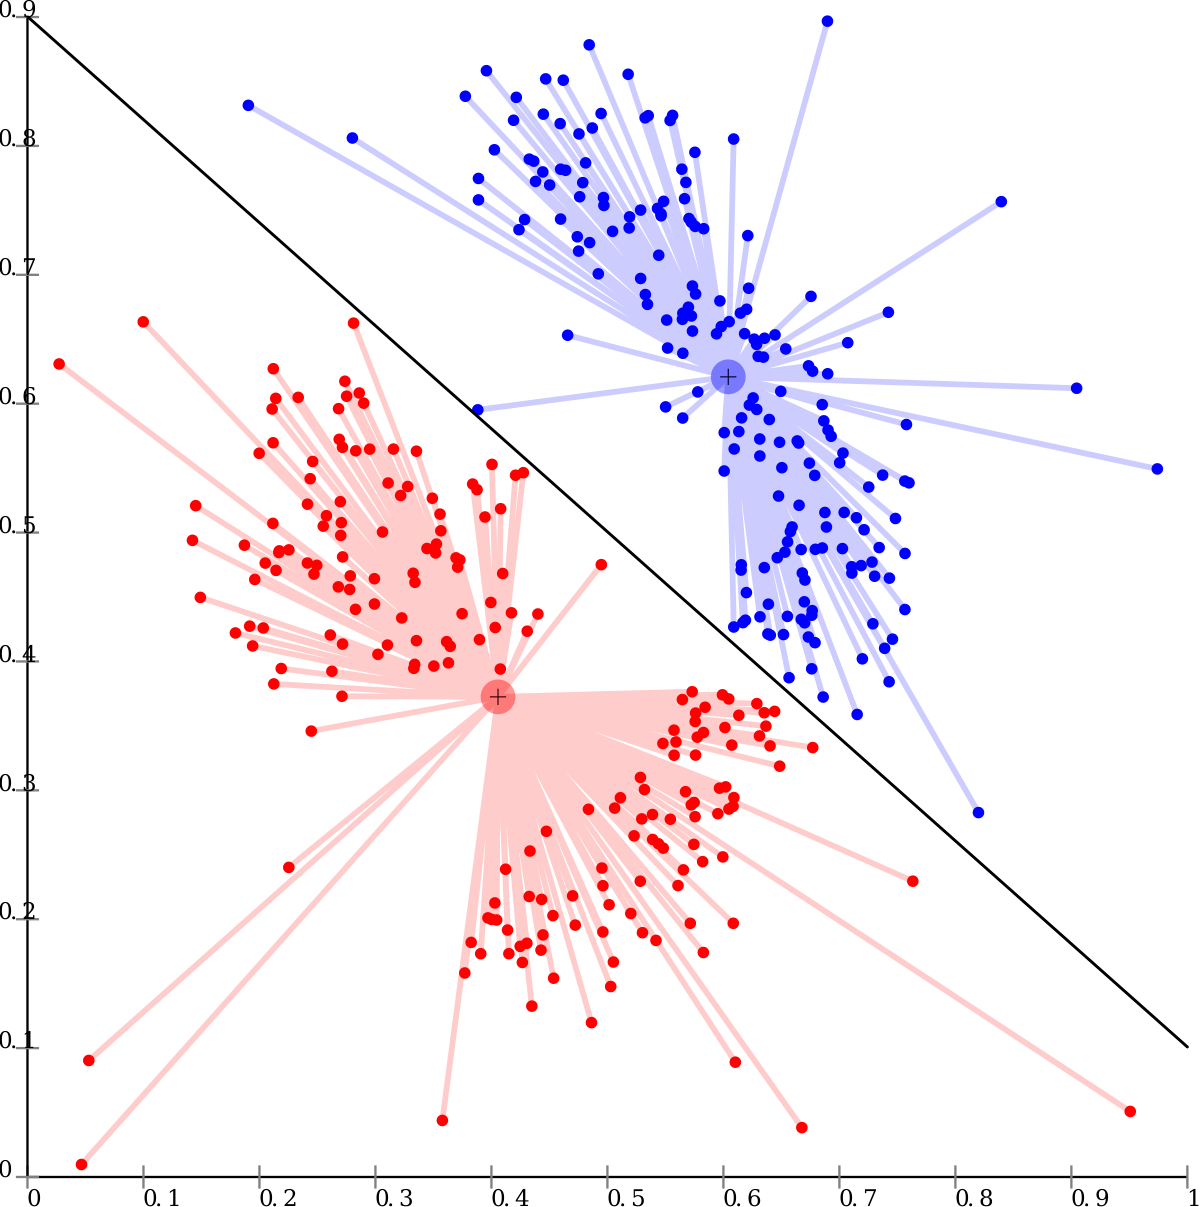
\includegraphics[scale=0.15]{3_6}
    \centering
\end{figure}
\paragraph{Superparamagnetic Clustering}
This method is inspired by statistical mechanics, it does not assume a-priori distributions
for the data, and groups spikes into clusters as a function of a single parameter: the
temperature.\\
It is at the base of the software realized by the group of Rodrigo Quian Quiroga
(University of Leicester, UK) called Wave Clus. This method is implemented as an
iteration (by Monte Carlo method) of a Potts model. The Potts model is a generalization
of the Ising model, where instead of having spins with values \(\pm\frac{1}{2}\), there
are \(q\) different states per particle.
\begin{itemize}
    \item The \(p\)-selected features of a generic \(i\)-th spike are represented by a
          point \(x_i\) in a \(p\)-dimensional phase space. Then, let's define the
          interaction strength between two points \(x_i\) and \(x_j\):
          \begin{align*}
              J_{ij}=
              \begin{cases}
                  \begin{matrix}
                      \frac{1}{K}\exp{\biggl(-\frac{\|x_i-x_j\|^2}{2a^2}\biggr)} &  & \text{if}\,x_i\,\text{is a nearest neighbor of}\,x_j \\
                      0                                                          &  & \text{else}
                  \end{matrix}
              \end{cases}
          \end{align*}
          where \(a\) is the average nearest-neighbor distance and \(K\) is the number
          of nearest neighbors. As a consequence, similar spikes will exhibit a strong
          interaction.
    \item At this point, a random state is assigned to each point \(x_i\) and \(N\)
          Monte Carlo iterations are run for different temperatures \(T\). A point \(x_i\)
          is randomly selected and its state is randomly changed to \(s_{new}\)
          (chosen between 1 and \(q\)). The probability that the nearest neighbors of \(x_i\)
          will change their state to \(s_{new}\) is given by:
          \begin{align*}
              p_{ij}=1-\exp{\biggl(-\frac{J_{ij}}{T}\delta_{s_i,s_j}\biggr)}
          \end{align*}
          This implies that close points will change their status together, forming
          clusters of spikes with similar shape. This observation can be quantified by
          measuring the point-to-point correlation \(\delta_{s_i,s_j}\) and defining
          \(x_i,x_j\) to be members of the same cluster if
          \(\delta_{s_i,s_j}\leq\theta\), for a given threshold \(\theta\).\\
          Moreover:
          \begin{itemize}
              \item \textbf{High temperatures} correspond to a low probability of changing
                    the state \(\Rightarrow\) states change randomly, thus no clusters
                    are formed (paramagnetic phase).
              \item \textbf{Low temperatures} correspond to a high probability of changing
                    to the same state, regardless of the interaction strength \(J_{ij}\)
                    \(\Rightarrow\) all states are changed to the same, thus all spikes
                    belong to the same cluster (ferromagnetic phase).
              \item \textbf{Medium temperatures} correspond to a phase in which only similar
                    spikes will change their state together, forming meaningful clusters
                    (superparamagnetic phase).
          \end{itemize}
\end{itemize}
\begin{figure}[H]
    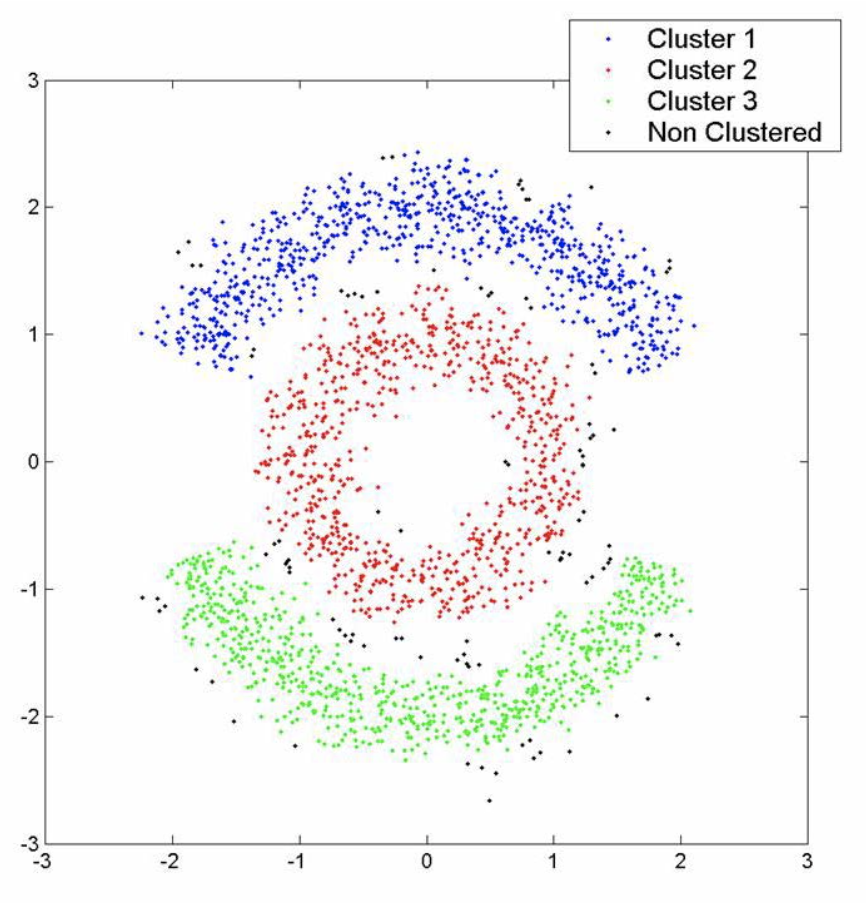
\includegraphics[scale=0.32]{3_7}
    \centering
\end{figure}
In this image some large size clusters corresponding to the optimal sorting can be
observed:
\begin{itemize}
    \item Clusters partially overlap
    \item They have a large variance
    \item The centers fall outside the clusters
    \item The distance between arbitrarily chosen points of the same cluster can
          be much larger than the distance between points in different clusters.
\end{itemize}

\subsection{Miscellanea}
In the following are reported some further remarks and considerations concerning
Spike Sorting.
\subsubsection{Spike Sorting issues}
The main issues when it comes to Spike Sorting are listed below:
\begin{itemize}
    \item \textbf{Electrode Drift:} waveforms of a given neuron vary over
          time and may be assigned to multiple clusters.
    \item \textbf{Tetrodes:} tetrode recordings can be exploited to improve
          spike sorting results, since they allow the visualization of single
          neurons from different positions.
    \item \textbf{Overlapping Spikes:} this phenomenon can be observed when
          two close-by neurons fire in synchrony or with a small delay. Still
          an open issue in Spike Sorting.
    \item \textbf{Bursting Cells:} a burst is the firing of a fast sequence
          of spikes by a neuron. Successive spikes in a burst may have decreasing
          amplitude and may be mistakenly considered as separate clusters.
\end{itemize}
\subsubsection{KiloSort}
Kilosort is a project whose aim is to develop a fully automated, scalable, and accurate
spike sorter, removing the burden of this task from researchers. It belongs to the
template matching class of Spike Sorting algorithms.\\
The main hypothesis of KiloSort is that spatial and temporal shapes of a waveform
provide all the information necessary to assign a given spike to a neuron. This
algorithm exploits template matching in both spike detection and spike clustering,
which are condensed into a single unified model describing the voltage \(V\) of channel
\(i\) at the time instant \(t\):
\begin{align*}
    V(i,t)=\sum_{k=1}^{N_{spike}}A_{\sigma(k)}(i,t-t_k)\cdot x(k) + noise
\end{align*}
with \(A_{\sigma(k)}(i,t-t_k)\) being the spike template for the \(k\)-th neuron
and \(x(k)\) the amplitude of the spike emitted by the \(k\)-th neuron. Hence, it
basically omits spike detection and PCA (both of these steps may discard potentially
useful information) and instead combines the identification of template waveforms and
associated spike times.
\subsubsection{Performance evaluation}
Different Spike Sorting methods can be compared by testing them on simultaneous
extracellular and intracellular recordings datasets, in a similar fashion with respect
to Spike Detection. Often, simulated datasets are used, where the identity of each
spike is known: it is important to create datasets that mimic as accurately as possible
the characteristics of real recordings in terms of noise distribution, spike features,
and so on.\\
The SpikeForest project aims at benchmarking and testing the finest and most recent
Spike Sorting algorithms.
